\documentclass{report}

\usepackage{graphicx}
\usepackage{algorithm}
\usepackage{array}
\usepackage{dsfont}
\usepackage{algpseudocode}
\usepackage{listings}
\usepackage{amsmath}
\usepackage{tikz}
\usepackage{pdfpages}
\usepackage{float}

\usetikzlibrary{automata, positioning, arrows}
\DeclareMathOperator{\rank}{rank}
\makeatletter
\newenvironment{sqcases}{%
  \matrix@check\sqcases\env@sqcases
}{%
  \endarray\right.%
}
\def\env@sqcases{%
  \let\@ifnextchar\new@ifnextchar
  \left\lbrack
  \def\arraystretch{1.2}%
  \array{@{}l@{\quad}l@{}}%
}
\makeatother

\usetikzlibrary{calc}


\input{/mnt/fa80f336-3342-4d78-8bfd-a43e434a2cda/Latex/preamble.tex}
\input{/mnt/fa80f336-3342-4d78-8bfd-a43e434a2cda/Latex/macros.tex}
\input{/mnt/fa80f336-3342-4d78-8bfd-a43e434a2cda/Latex/letterfonts.tex}

\title{\Huge{FU08 \-- Automata and Languages}\\Exercise 3}
\author{\huge{NGUYEN Tuan Dung}\\\huge{s1312004}}
\date{December 10, 2024}

\begin{document}

\maketitle

% Cau 1
\qs{Answer the following question}{
    Give DFAs accepting the following languages\\
    (Over the alphabet \{0,1\}):\\
    \newline
    a. The language of all strings ending in 00.\\
    b. The language of all strings with three consecutive 0's.
}

\sol{\newline
a. State definition:
\begin{itemize}
    \item $\mathrm{q}_{0}$: The string does not contain anything, waiting for input.
    \item $\mathrm{q}_{1}$: The string ends in 0.
    \item $\mathrm{q}_{2}$: The string ends in 00. $\mathrm{q}_{2} \in \mathds{F}$
\end{itemize}
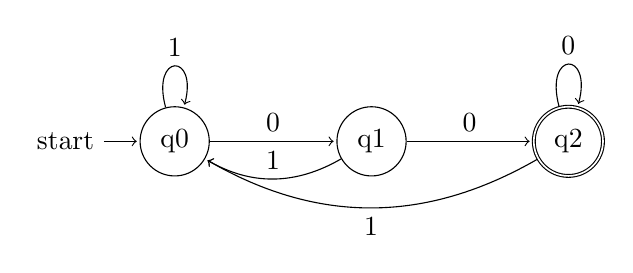
\begin{tikzpicture}[shorten >=1pt, node distance=2.5cm, on grid, auto]
    \node[state, initial] (q0)   {q0}; 
    \node[state] (q1) [right=of q0] {q1}; 
    \node[state, accepting] (q2) [right=of q1] {q2}; 

    \path[->]
    (q0) edge [loop above] node {1} ()
          edge node {0} (q1)
    (q1) edge node {0} (q2)
          edge [bend left, above] node {1} (q0)
    (q2) edge [loop above] node {0} ()
          edge [bend left, below] node {1} (q0);
\end{tikzpicture}
\newline
b. State definition:
\begin{itemize}
    \item $\mathrm{q}_0$: The string does not contain anything, waiting for input.
    \item $\mathrm{q}_1$: The string contains 0.
    \item $\mathrm{q}_2$: The string contains 00 (consecutively).
    \item $\mathrm{q}_3$: The string contains 000 (consecutively). $\mathrm{q}_3 \in \mathds{F}$
\end{itemize}
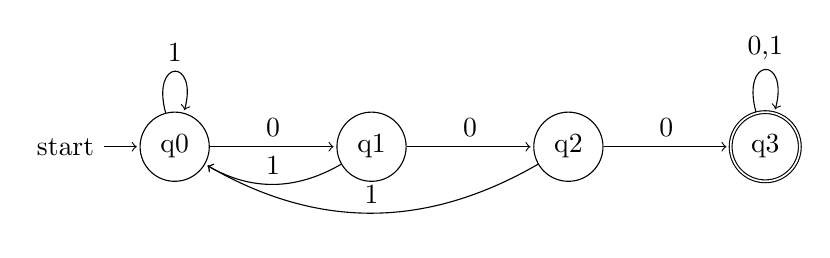
\begin{tikzpicture}[shorten >=1pt, node distance=2.5cm, on grid, auto]
    \node[state, initial] (q0)   {q0}; 
    \node[state] (q1) [right=of q0] {q1}; 
    \node[state] (q2) [right=of q1] {q2}; 
    \node[state, accepting] (q3) [right=of q2] {q3}; 

    \path[->]
    (q0) edge [loop above] node {1} ()
          edge node {0} (q1)
    (q1) edge node {0} (q2)
          edge [bend left, above] node {1} (q0)
    (q2) edge node {0} (q3)
          edge [bend left, above] node {1} (q0)
    (q3) edge [loop above] node {0,1} ();
\end{tikzpicture}
}
\newline

% Cau 2
\qs{Answer the fullowing question}{
    For $\sum = \{\mathrm{a},\mathrm{b}\}$, construct DFAs accepting the following languages:\\
    \newline
    a. The language of all strings with exactly one a.\\
    b. The language of all strings with at least one a.\\
    c. The language of all strings with no more than three a's.
}

\sol{\newline
a. State defintion:
\begin{itemize}
    \item $\mathrm{q}_{0}$: The string does not contain anything, waiting for input.
    \item $\mathrm{q}_{1}$: The string contains exactly one a. $\mathrm{q}_{1} \in \mathds{F}$
    \item $\mathrm{q}_{2}$: The string contains more than one a.
\end{itemize}
\begin{tikzpicture}[shorten >=1pt, node distance=2.5cm, on grid, auto]
    \node[state, initial] (q0) {q0};
    \node[state, accepting] (q1) [right=of q0] {q1};
    \node[state] (q2) [right=of q1] {q2};

    \path[->]
    (q0) edge [loop above] node {b} ()
         edge node {a} (q1)
    (q1) edge [loop above] node {b} ()
         edge node {a} (q2)
    (q2) edge [loop above] node {a,b} ()
\end{tikzpicture}
\newline
\newline
b. State definition:
\begin{itemize}
    \item $\mathrm{q}_{0}$: The string does not contain anything, waiting for input.
    \item $\mathrm{q}_{1}$: The string contains 0. $\mathrm{q}_1 \in \mathds{F}$
\end{itemize}
\begin{tikzpicture}[shorten >=1pt, node distance=2.5cm, on grid, auto]
    \node[state, initial] (q0)   {q0}; 
    \node[state, accepting] (q1) [right=of q0] {q1}; 

    \path[->]
    (q0) edge [loop above] node {b} ()
          edge node {a} (q1)
    (q1) edge [loop above] node {a,b} ()
\end{tikzpicture}
\newline
\newline
c. State definition:
\begin{itemize}
    \item $\mathrm{q}_{0}$: The string does not contain anything, waiting for input. $\mathrm{q}_{0} \in \mathds{F}$
    \item $\mathrm{q}_{1}$: The string contains one a. $\mathrm{q}_{1} \in \mathds{F}$
    \item $\mathrm{q}_{2}$: The string contains two a's. $\mathrm{q}_{2} \in \mathds{F}$
    \item $\mathrm{q}_{3}$: The string contains three a's. $\mathrm{q}_{3} \in \mathds{F}$
    \item $\mathrm{q}_{4}$: The string contains more than three a's.
\end{itemize}
\begin{tikzpicture}[shorten >=1pt, node distance=2.5cm, on grid, auto]
    \node[state, initial, accepting] (q0) {q0};
    \node[state, accepting] (q1) [right=of q0] {q1}; 
    \node[state, accepting] (q2) [right=of q1] {q2}; 
    \node[state, accepting] (q3) [right=of q2] {q3}; 
    \node[state] (q4) [right=of q3] {q4}; 

    \path[->]
    (q0) edge [loop above] node {b} ()
         edge node {a} (q1)
    (q1) edge [loop above] node {b} ()
         edge node {a} (q2)
    (q2) edge [loop above] node {b} ()
         edge node {a} (q3)
    (q3) edge [loop above] node {b} ()
         edge node {a} (q4)
    (q4) edge [loop above] node {a,b} ()
    
\end{tikzpicture}
}


\end{document}
